\documentclass{minimal}
\usepackage{tikz}

\newcommand{\radius}{R}
\newcommand{\separation}{d}
\newcommand{\stiffness}{k_f}
\newcommand{\boltzmann}{k_B}
\newcommand{\temp}{T}
\newcommand{\onConst}{k_\text{on}}
\newcommand{\offConst}{k_\text{off}}
\newcommand{\refForce}{f_0}
\newcommand{\receptorDensity}{N_T}
\newcommand{\receptorNumber}{N_R}
\newcommand{\appliedRot}{\Omega_f}
\newcommand{\appliedVel}{V_f}
\newcommand{\velFriction}{\xi_V}
\newcommand{\rotFriction}{\xi_\omega}
\newcommand{\compliance}{\Gamma}
\newcommand{\width}{w}
\newcommand{\viscosity}{\mu}

\newcommand{\ndSeparation}{d'}
\newcommand{\ndAppliedRot}{\omega_f}
\newcommand{\ndAppliedVel}{v_f}
\newcommand{\ndOnConst}{\kappa}
\newcommand{\onForceScale}{\eta}
\newcommand{\offForceScale}{\delta}
\newcommand{\ndVelFriction}{\eta_v}
\newcommand{\ndRotFriction}{\eta_\omega}

\newcommand{\ITA}[1]{\textalpha\textsubscript{#1}}
\newcommand{\ITB}[1]{\textbeta\textsubscript{#1}}


\begin{document}
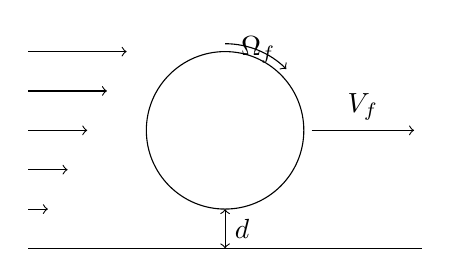
\begin{tikzpicture}
  \newcommand{\dist}{0.5}
  \newcommand{\Length}{2.5}
  \newcommand{\slope}{0.5}
  \newcommand{\buff}{0.1}

  % Draws the wall and the platelet
  \draw (-\Length, 0) -- (\Length, 0);
  \draw (0, 1+\dist) circle [radius = 1];
  \draw[<->] (0, 0) -- node[right] {$\separation$} (0, \dist);
  \draw[->] (1+\buff, 1+\dist) -- node[above] {$\appliedVel$}
            (\Length-\buff, 1+\dist);

  % Computations necessary to draw the applied rotation annotation
  \draw[->] (0, 2+\buff+\dist) arc [start angle=90, end angle=45,
                                    radius=1+\buff]
                               node[midway] {$\appliedRot$};

  % Draws the arrows showing the shear flow
  \foreach \y in {0.5, 1, 1.5, 2, 2.5}
     \draw[->] (-\Length, \y) -- (-\Length + \slope*\y, \y);
\end{tikzpicture}
\end{document}